\begin{tframe}{Adversarial Training}

The method of training used for this case is inspired by the one proposed by [1].

\vspace{0.1in}

In [1], the objective function is modified to include adversarial examples in the training phase, by doing a weighted sum of the loss for the clean and the adversarial examples:
$$ 	\tilde{J}(\theta, x, y) = \alpha J(\theta, x, y) + ( 1 - \alpha)J(\theta, x + \epsilon sign(\nabla_{x}J(\theta, x, y)), y) $$

\vspace{0.1in}

In the implemented method, the same principle is applied only to the computing of the gradients wrt the weights in the backpropagation, so that the direction chosen for the next step will also take into consideration adversarial examples. 

\vspace{0.1in}

In the implementation, $ \alpha = 0.5 $

\end{tframe}

\begin{tframe}{Adversarial Training}

\begin{center}
  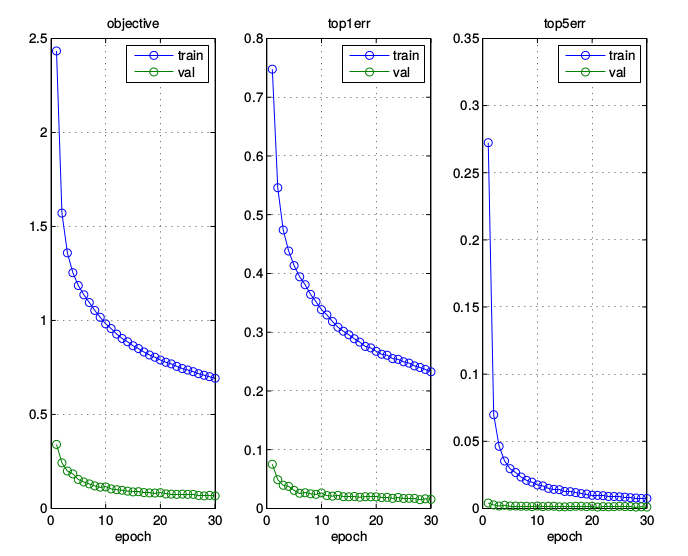
\includegraphics[width=0.7\textwidth]{img/train-adv.png}
	\label{train-mix} 
\end{center}

\end{tframe}

\begin{tframe}{Adversarial Training}

The tests were carried out as for the standard and mixed training.

\begin{table}[h]
\centering
\begin{tabular}{@{}lll@{}}
\toprule
                               & Clean & Adversarial \\ \midrule
Correctly Predicted            & 97.97 & 77.80       \\
Error                          & 2.03  & 22.20       \\
Confidence                     & 96.03 & 79.05       \\
Correctly Predicted Confidence & 96.69 & 82.55       \\
Error Confidence               & 64.23 & 66.79       \\ \bottomrule
\end{tabular}
\end{table}

\end{tframe}